\section{正文补充图}

本附录保存正文因 30 页限制移出的探索性、流程性和解释性图。所有图均由本轮正式 JSON/CSV 重新生成。

\begin{figure}[htbp]
\centering
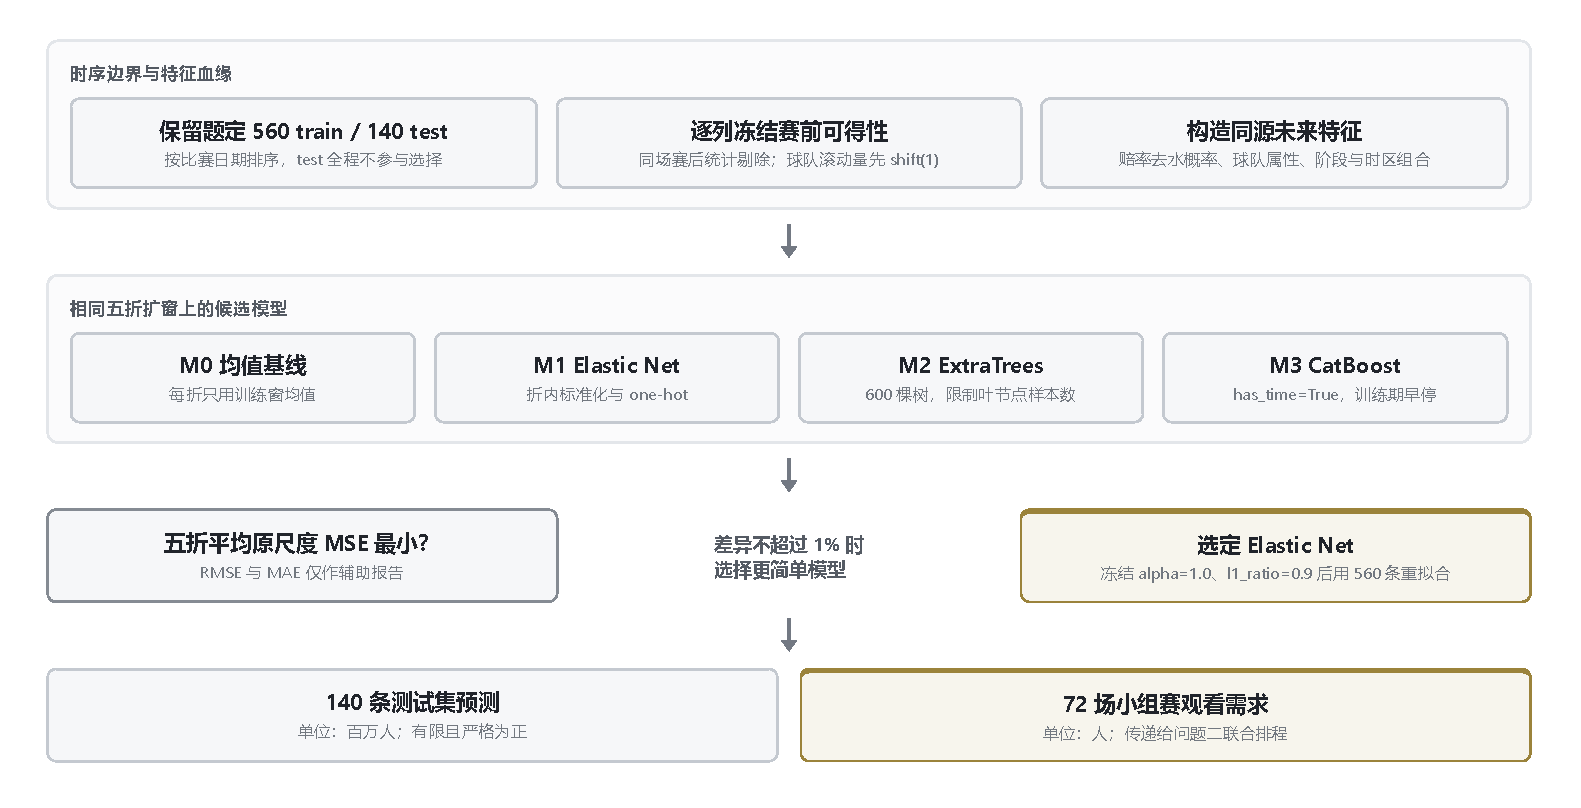
\includegraphics[width=0.85\textwidth,height=0.55\textheight,keepaspectratio]{../figures/fig_flow_q1.pdf}
\caption{问题一求解流程}\label{fig:flow-q1}
\end{figure}

\begin{figure}[htbp]
\centering
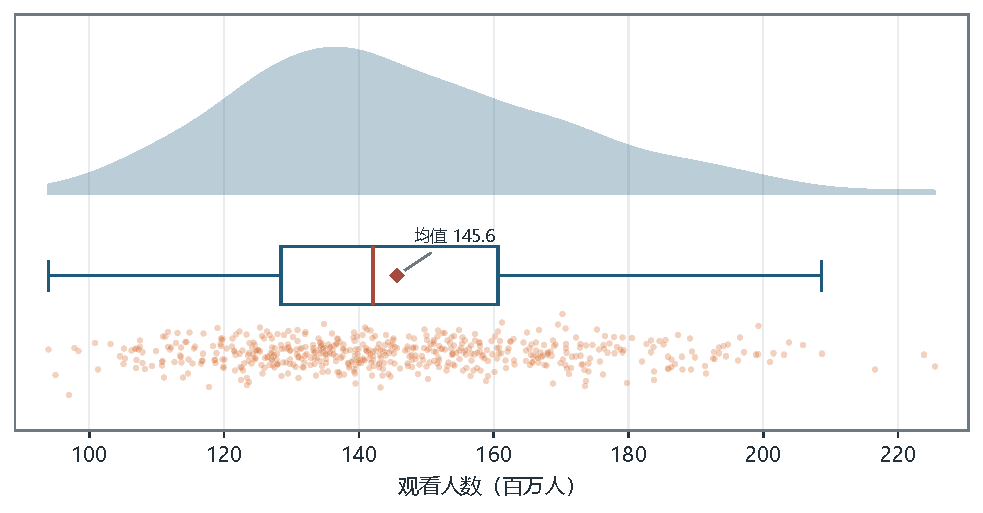
\includegraphics[width=0.85\textwidth,height=0.72\textheight,keepaspectratio]{../figures/fig_q1_target_raincloud.pdf}
\caption{训练集观看人数分布与长尾特征}\label{fig:q1-target-raincloud}
\end{figure}

\begin{figure}[htbp]
\centering
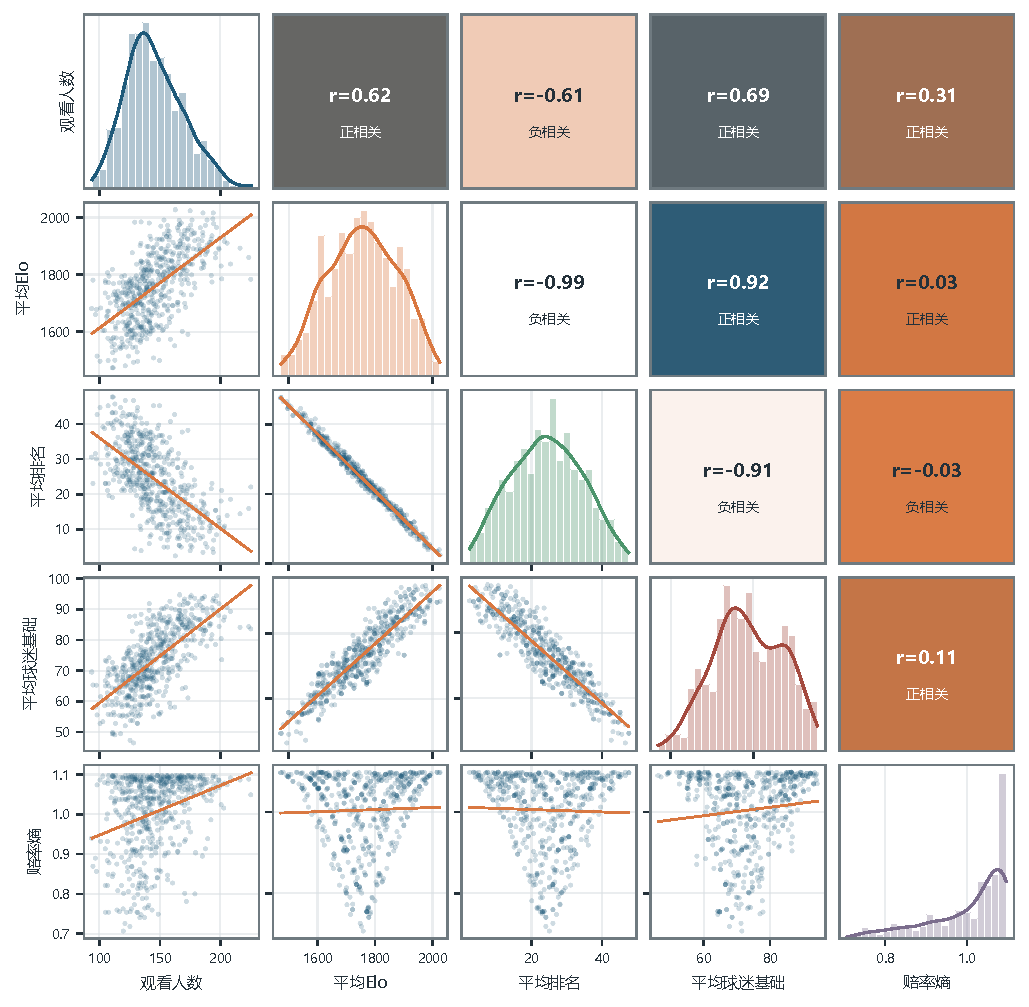
\includegraphics[width=0.85\textwidth,height=0.72\textheight,keepaspectratio]{../figures/fig_q1_feature_pairplot.pdf}
\caption{问题一核心赛前特征成对关系}\label{fig:q1-feature-pairplot}
\end{figure}

\begin{figure}[htbp]
\centering
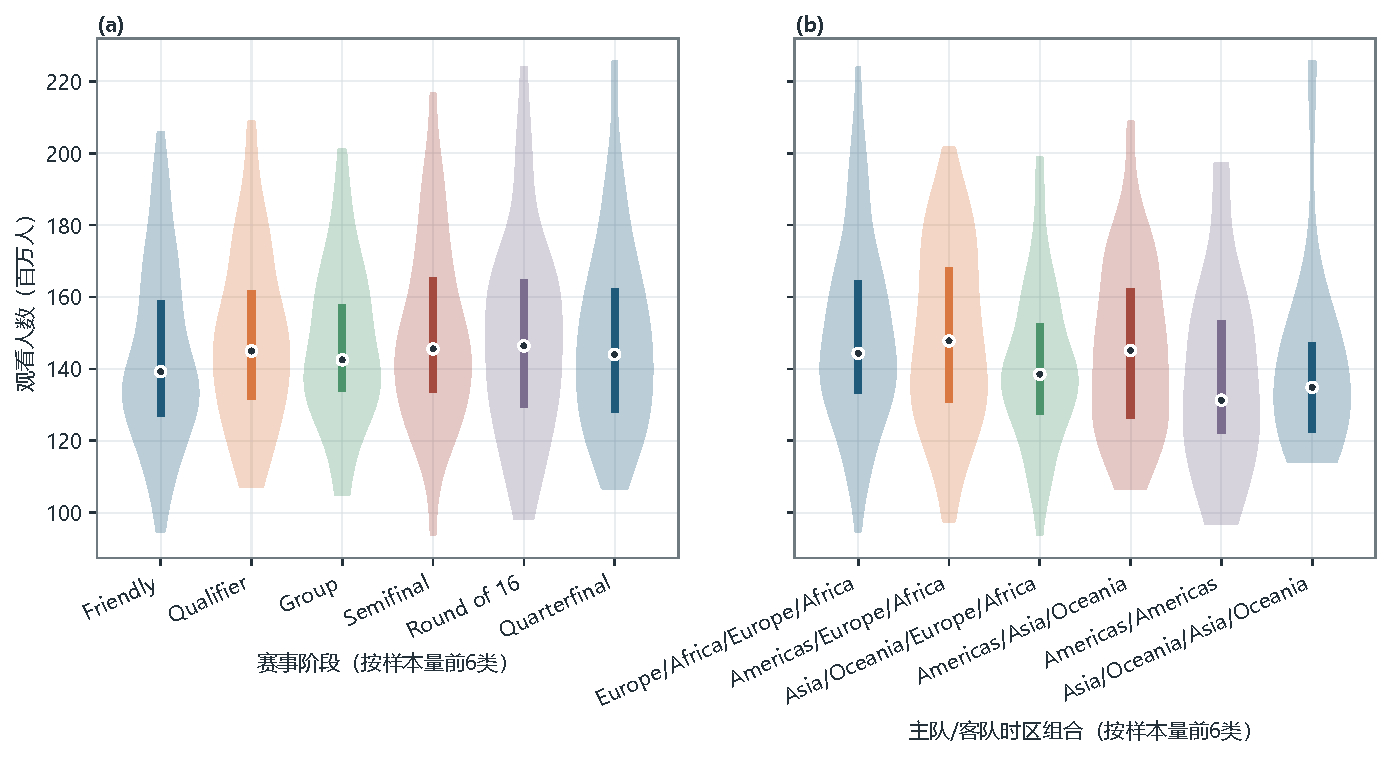
\includegraphics[width=0.85\textwidth,height=0.72\textheight,keepaspectratio]{../figures/fig_q1_stage_timezone_violin.pdf}
\caption{赛事阶段与时区组合下观看人数异质性}\label{fig:q1-stage-timezone-violin}
\end{figure}

\begin{figure}[htbp]
\centering
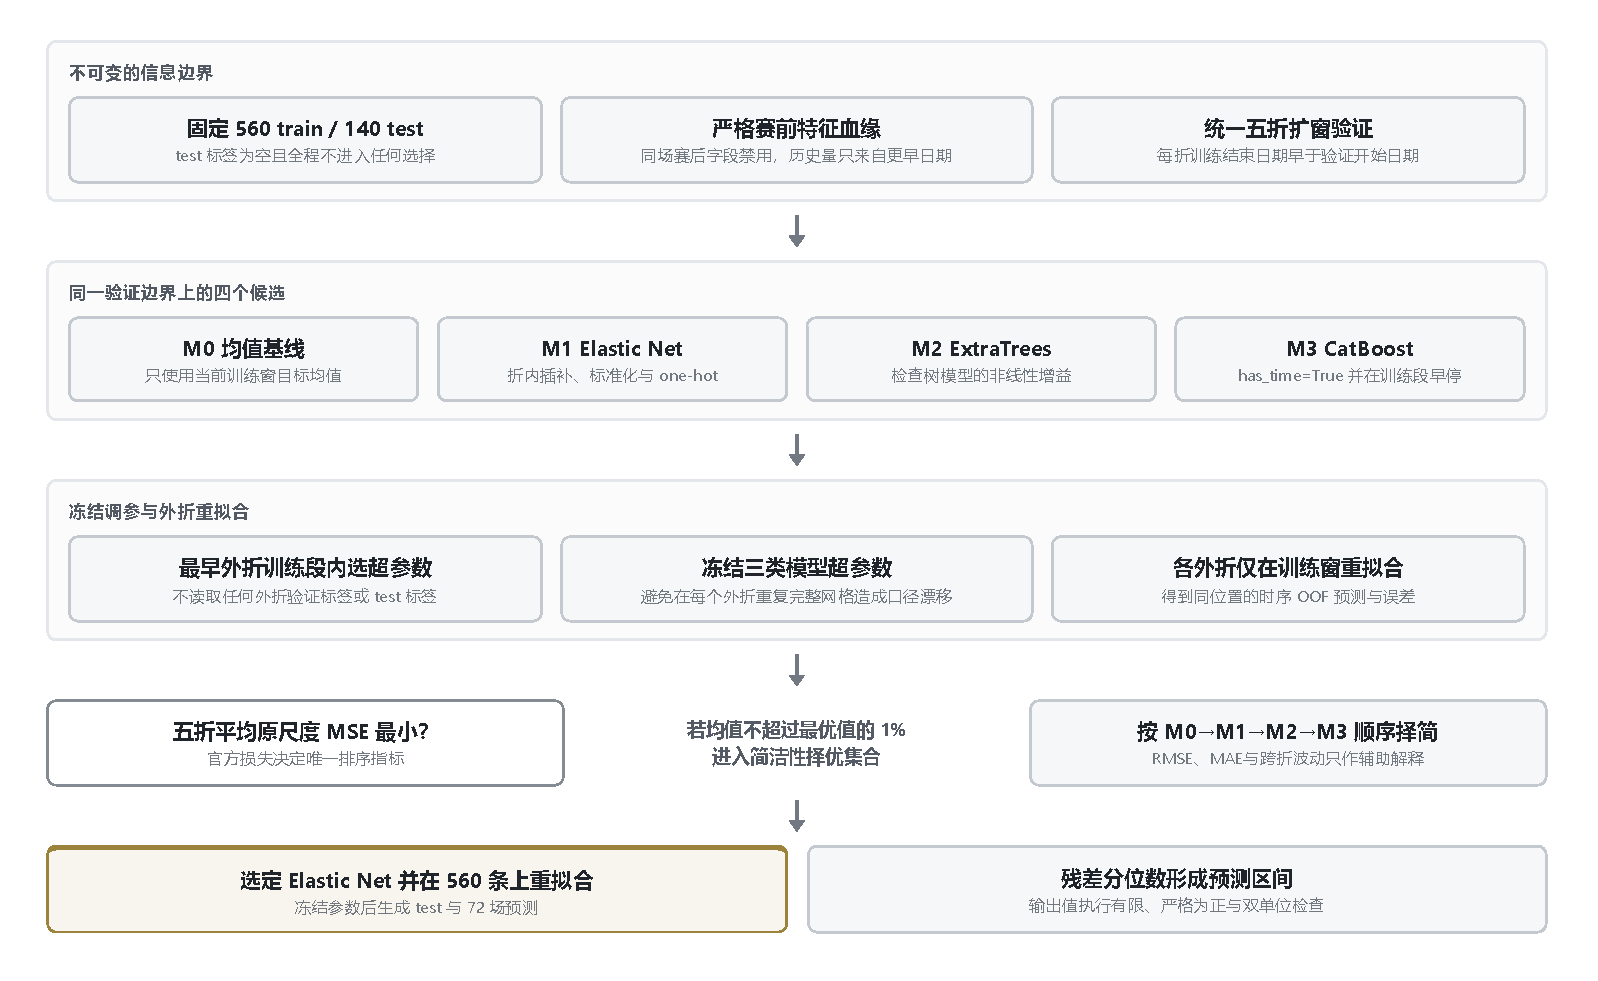
\includegraphics[width=0.85\textwidth,height=0.55\textheight,keepaspectratio]{../figures/fig_model_decision.pdf}
\caption{预测模型选择流程}\label{fig:model-decision}
\end{figure}

\begin{figure}[htbp]
\centering
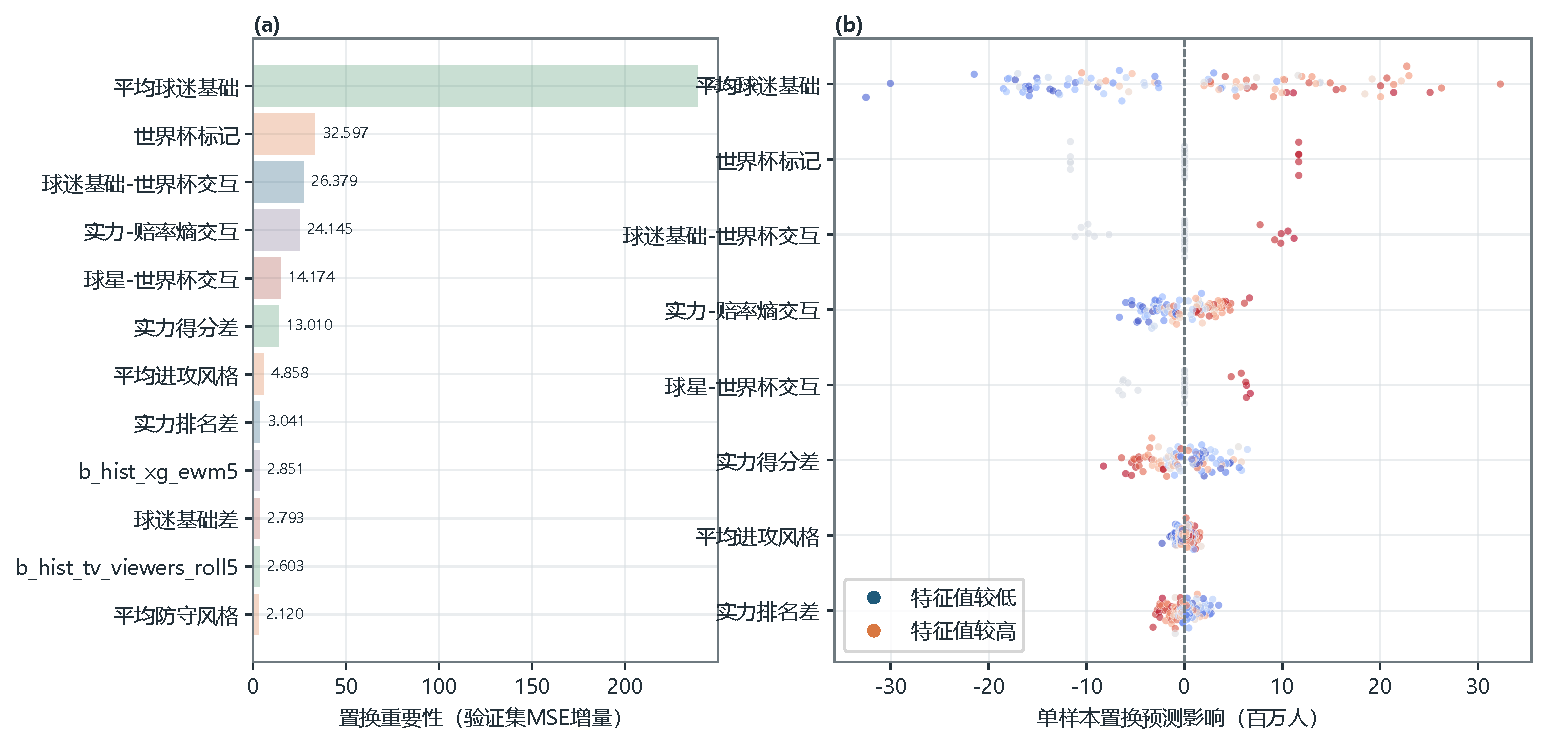
\includegraphics[width=0.85\textwidth,height=0.72\textheight,keepaspectratio]{../figures/fig_q1_shap_summary.pdf}
\caption{Elastic Net置换重要性与单样本预测影响}\label{fig:q1-shap-summary}
\end{figure}

\begin{figure}[htbp]
\centering
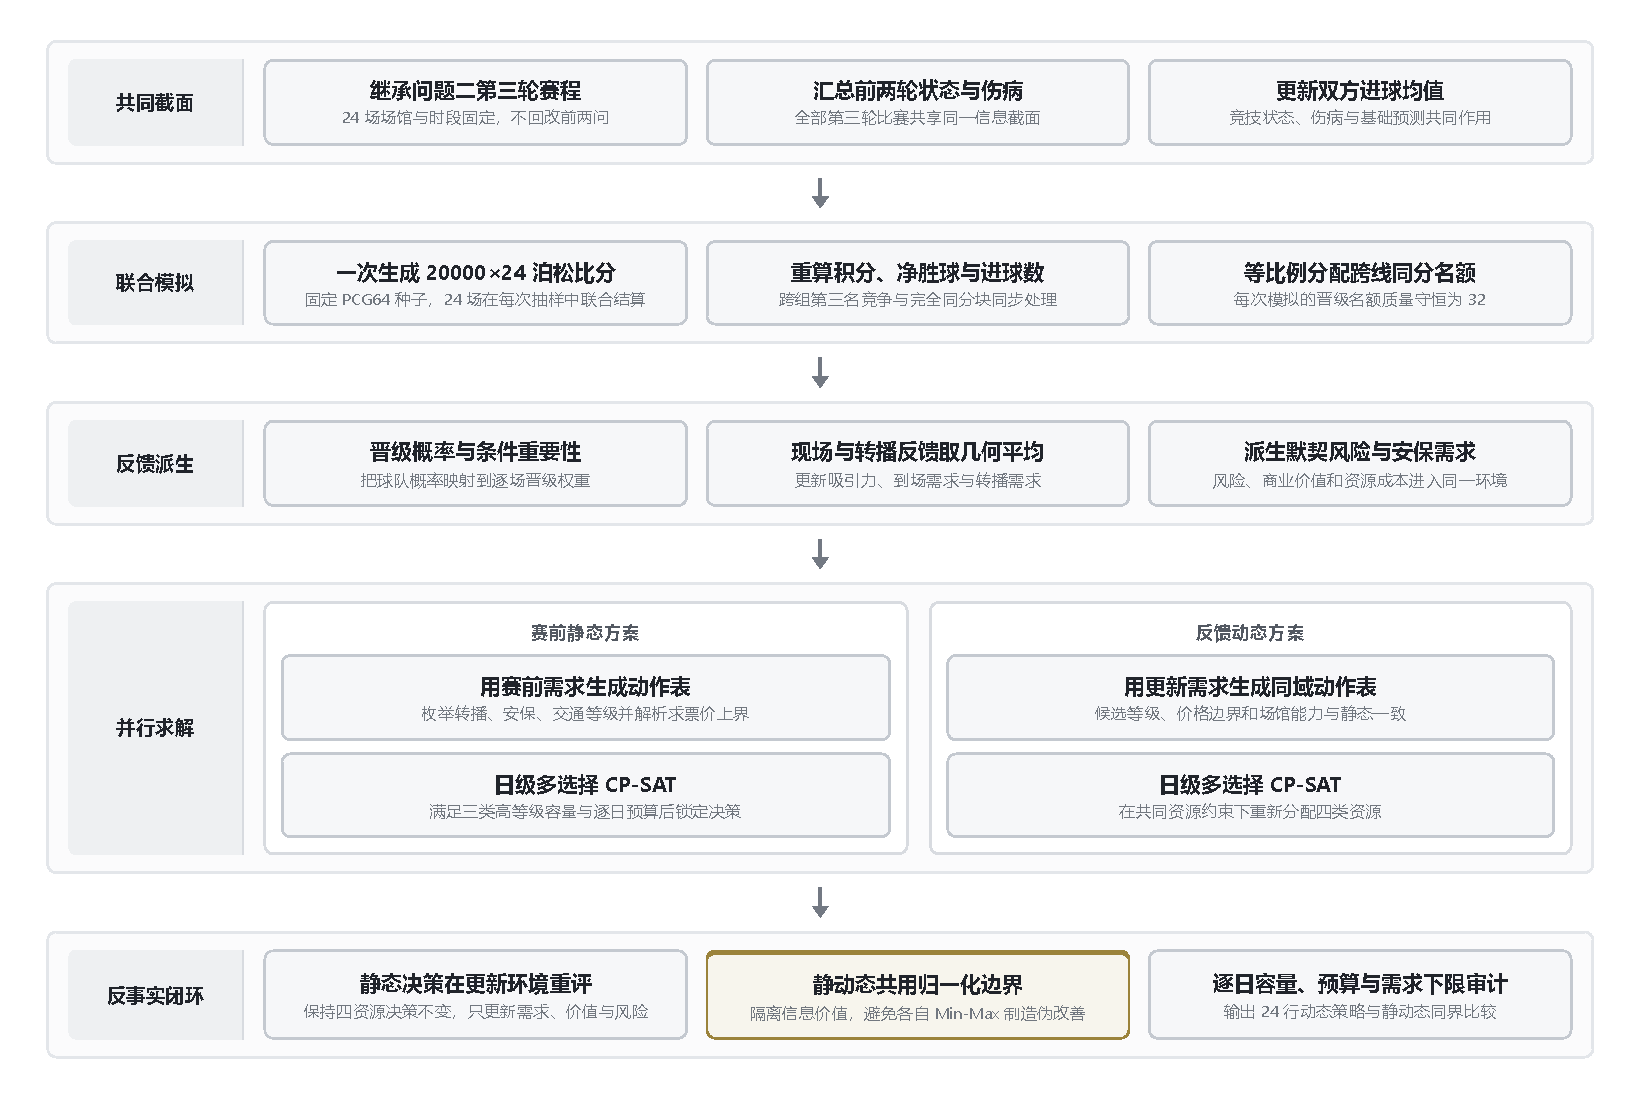
\includegraphics[width=0.88\textwidth,height=0.58\textheight,keepaspectratio]{../figures/fig_flow_q3.pdf}
\caption{问题三共同信息截面与静动态同界比较流程}\label{fig:flow-q3}
\end{figure}

\begin{figure}[htbp]
\centering
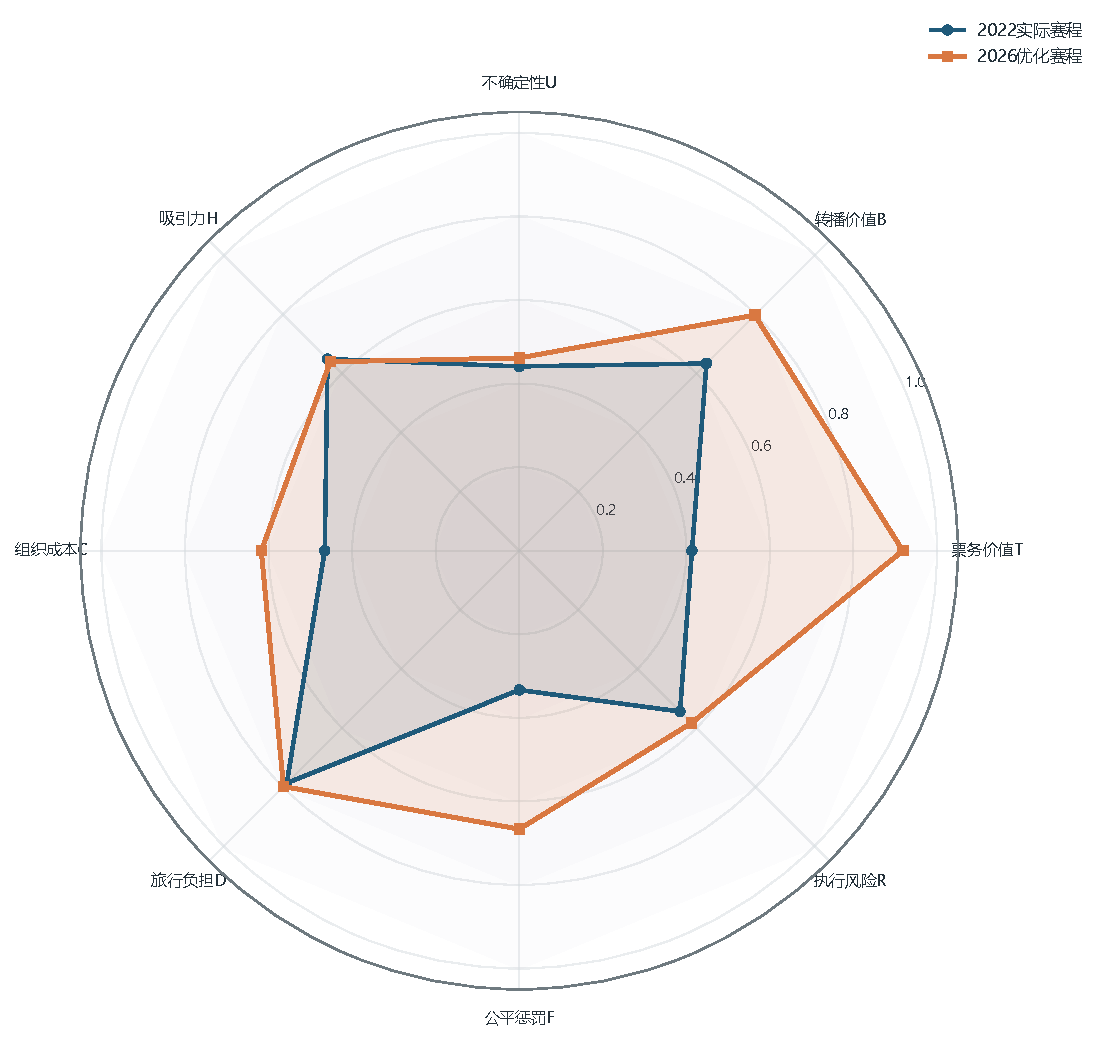
\includegraphics[width=0.85\textwidth,height=0.72\textheight,keepaspectratio]{../figures/fig_q4_metric_radar.pdf}
\caption{同构代理层的指标轮廓}\label{fig:q4-metric-radar}
\end{figure}
